\documentclass[tikz,border=4pt]{standalone}
\usepackage{amsmath,amssymb,bm}
\usepackage[T1]{fontenc}
\usepackage{newtxtext,newtxmath}
\usepackage{microtype}
\usepackage{tikz}
\usetikzlibrary{arrows.meta,positioning,calc,fit,backgrounds,decorations.pathreplacing,shadows.blur}

% =================== palette ===================
\definecolor{headFill}{HTML}{F7FAFC}
\definecolor{headLine}{HTML}{172033}
\definecolor{ink}     {HTML}{172033}
\definecolor{mutedInk}{HTML}{4B5565}
\definecolor{qkC}     {HTML}{B91C1C}
\definecolor{qkFill}  {HTML}{FEE2E2}
\definecolor{ovC}     {HTML}{0B7285}
\definecolor{ovFill}  {HTML}{E3F3F6}
\definecolor{saeC}    {HTML}{46378A}
\definecolor{saeFill} {HTML}{EEEAF8}
\definecolor{featHi}  {HTML}{D99A1E}
\definecolor{featHiD} {HTML}{7A4F08}

\tikzset{
  >=Latex,
  every node/.append style={line join=round},
  attnBox/.style    ={draw=none, fill=none, inner sep=6mm},
  inner/.style      ={font=\normalsize, inner sep=2pt, align=center, text=ink},
  nodeQK/.style     ={draw=qkC, line width=0.85pt, rounded corners=2.2pt,
                      fill=qkFill, font=\normalsize\bfseries, text=qkC,
                      inner sep=3pt, minimum height=6mm, minimum width=14mm,
                      align=center},
  nodeOV/.style     ={draw=ovC, line width=0.85pt, rounded corners=2.2pt,
                      fill=ovFill, font=\normalsize\bfseries, text=ovC,
                      inner sep=3pt, minimum height=6mm, minimum width=14mm,
                      align=center},
  outnode/.style    ={font=\normalsize\bfseries, text=ink, inner sep=2pt},
  xnode/.style      ={font=\normalsize, text=ink, inner sep=2pt},
  flow/.style       ={->, line width=0.78pt, ink, line cap=round},
  qkflow/.style     ={->, line width=0.95pt, qkC, line cap=round},
  ovflow/.style     ={->, line width=0.95pt, ovC, line cap=round},
  saeBox/.style     ={draw=saeC, line width=0.95pt, rounded corners=4pt,
                      fill=saeFill, inner sep=3mm},
  feat/.style       ={draw=saeC!62, line width=0.45pt, fill=white,
                      minimum width=5mm,minimum height=5mm,
                      inner sep=0pt,font=\scriptsize\bfseries},
  featHi/.style     ={draw=featHi, line width=1.15pt, fill=featHi!24,
                      minimum width=5mm,minimum height=5mm,
                      inner sep=0pt,font=\scriptsize,text=featHiD},
  brace/.style      ={decorate,decoration={brace,amplitude=6pt,raise=2pt}},
  braceMirror/.style={decorate,decoration={brace,amplitude=6pt,raise=2pt,mirror}},
  panel/.style 2 args ={draw=#1, line width=0.95pt, rounded corners=4pt, fill=#2,
                        inner sep=3.2mm, font=\normalsize, text=ink},
}

\begin{document}
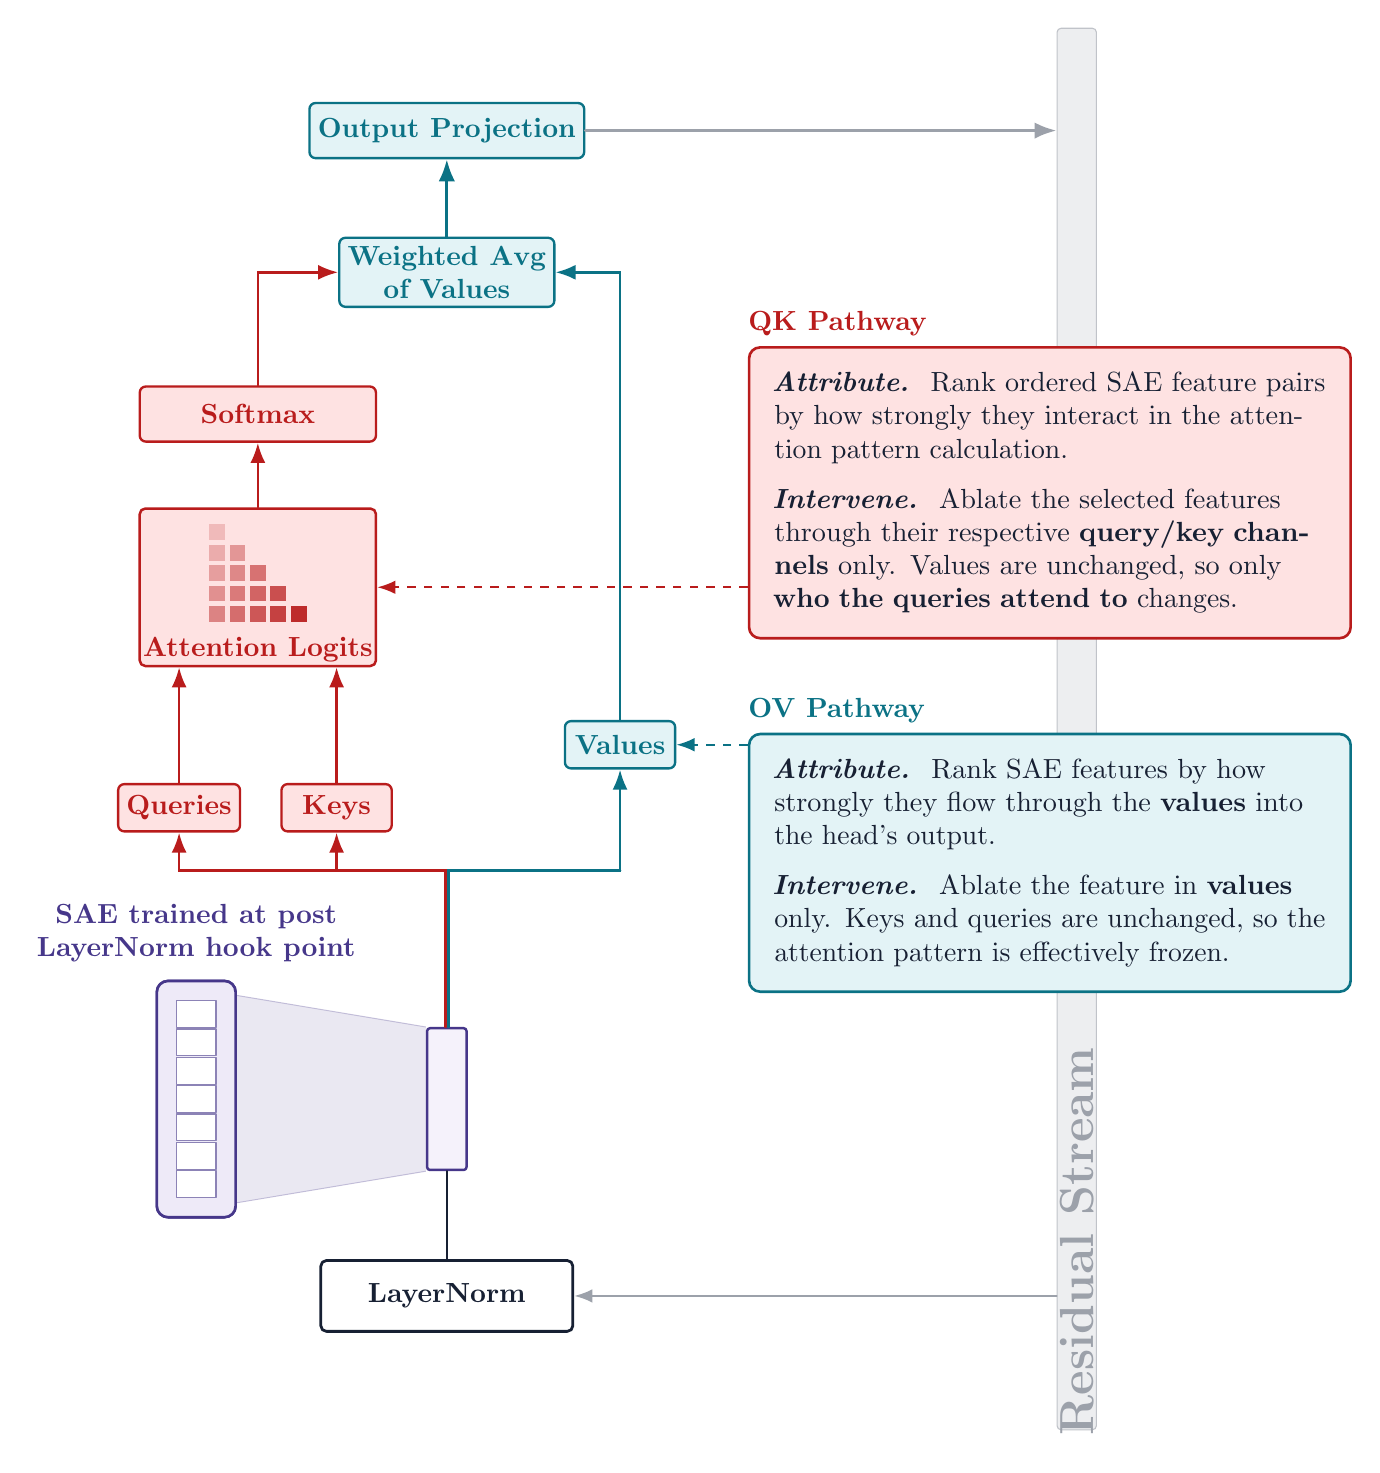
\begin{tikzpicture}[x=1mm,y=1mm]

% ============================================================
% Inner-head nodes (absolute coords)
% ============================================================
\node[nodeQK]   (queries) at (-22,34) {Queries};
\node[nodeQK]   (keys)    at (-2,34)  {Keys};
\node[nodeOV]   (values)  at (34,42)  {Values};
% attention logits box (with the causal attention heatmap inside)
\node[draw=qkC,line width=0.9pt,rounded corners=2pt,fill=qkFill,
      minimum width=30mm,minimum height=20mm,inner sep=1mm]
      (logits) at (-12,62) {};
\node[font=\normalsize\bfseries,qkC,anchor=south,inner sep=1pt]
  at ([yshift=0.3mm]logits.south) {Attention Logits};

\pgfmathsetmacro{\HC}{2.6}
\foreach \r in {0,...,4} {%
  \foreach \c in {0,...,4} {%
    \pgfmathtruncatemacro{\active}{\c <= \r ? 1 : 0}%
    \pgfmathsetmacro{\op}{\active * (0.20 + 0.18*\c + 0.07*(\r-\c))}%
    \pgfmathsetmacro{\xc}{(\c-2)*\HC}%
    \pgfmathsetmacro{\yc}{1.8 + (2-\r)*\HC}%
    \fill[qkC,opacity=\op]
      ([xshift=\xc mm-1mm,yshift=\yc mm-1mm]logits.center)
      rectangle
      ([xshift=\xc mm+1mm,yshift=\yc mm+1mm]logits.center);
  }%
}

% softmax (small labeled box, no heatmap)
\node[nodeQK,minimum width=30mm,minimum height=7mm]
      (softmax) at (-12,84) {Softmax};

\node[nodeOV]   (wavg)    at (12,102) {Weighted Avg\\ of Values};
\node[nodeOV,minimum width=25mm,minimum height=7mm]
      (oproj)   at (12,120) {Output Projection};

% --- arrows inside head ---
\coordinate (jx) at (12,26);
\coordinate (jxQK) at ([xshift=-0.18mm]jx);
\coordinate (jxOV) at ([xshift=0.18mm]jx);
\draw[qkflow] (jxQK) -| (keys.south);
\draw[qkflow] (jxQK) -| (queries.south);
\draw[ovflow] (jxOV) -| (values.south);

\draw[qkflow] (keys.north)    -- (keys.north    |- logits.south);
\draw[qkflow] (queries.north) -- (queries.north |- logits.south);

\draw[qkflow] (logits.north) -- (softmax.south);

\draw[qkflow] (softmax.north) -- ++(0,3) |- (wavg.west);
\draw[ovflow] (values.north) |- (wavg.east);
\draw[ovflow,line width=1.1pt] (wavg.north) -- (oproj.south);

% ============================================================
% Head outline
% ============================================================
\coordinate (xTop)   at (12,16);
\coordinate (outTop) at (12,124);
\begin{scope}[on background layer]
  \node[attnBox,
        fit=(keys)(values)(logits)(softmax)(wavg)(xTop)(outTop)] (head) {};
\end{scope}

% ============================================================
% Below the head: LayerNorm on the main flow, then a tall
% post-LN activation block. The SAE is shown to the side as
% the tall block "expanded" into its sparse feature vector.
% ============================================================
% LayerNorm block in the main forward pass
\node[draw=headLine,line width=1pt,rounded corners=2pt,fill=white,
      minimum width=32mm,minimum height=9mm,font=\normalsize\bfseries,text=ink]
      (ln1) at (12,-28) {LayerNorm};

% Greyed residual stream lane feeding into LN and receiving the head output.
\coordinate (residIn)  at (92,-28);
\coordinate (residOut) at (92,120);
\begin{scope}[on background layer]
  \node[draw=mutedInk!35,fill=mutedInk!10,minimum width=5mm,minimum height=178mm,
        rounded corners=1.5pt,anchor=center] (residBar) at (92,44) {};
\end{scope}
\node[font=\LARGE\bfseries,text=mutedInk!55,rotate=90,anchor=center]
  at ([yshift=24mm]residBar.south) {Residual Stream};
\draw[->,line width=0.8pt,mutedInk!55,line cap=round]
  (residBar.west |- ln1.east) -- (ln1.east);
\draw[->,line width=1.1pt,mutedInk!55,line cap=round]
  (oproj.east) -- (residBar.west |- oproj.east);

% Tall post-LN activation block (taller than wide).
\node[draw=saeC,line width=0.9pt,rounded corners=1pt,fill=saeFill!60,
      minimum width=5mm,minimum height=18mm,inner sep=0pt]
      (postLNvec) at (12,-3) {};

% main flow lines (no arrowheads -- the split arrows above carry the direction)
\draw[line width=0.8pt,ink,line cap=round] (ln1.north) -- (postLNvec.south);
\draw[line width=0.95pt,qkC,line cap=round]
  ([xshift=-0.18mm]postLNvec.north) -- (jxQK) -- (keys.south |- jx);
\draw[line width=0.95pt,ovC,line cap=round]
  ([xshift=0.18mm]postLNvec.north) -- (jxOV) -- (values.south |- jx);

% External SAE box on the LEFT side: the same activation, "expanded" into
% its sparse feature decomposition. Vertical column of features.
\node[saeBox,minimum width=10mm,minimum height=30mm,
      left=24mm of postLNvec.west,anchor=east] (sae) {};

% shaded expansion from the tall activation block out to the SAE box
\begin{scope}[on background layer]
  \fill[saeC!38,opacity=0.30]
    (postLNvec.north west) -- ([yshift=-2mm]sae.north east) --
    ([yshift=2mm]sae.south east) -- (postLNvec.south west) -- cycle;
  \draw[saeC!55,opacity=0.55,line width=0.35pt]
    (postLNvec.north west) -- ([yshift=-2mm]sae.north east);
  \draw[saeC!55,opacity=0.55,line width=0.35pt]
    (postLNvec.south west) -- ([yshift=2mm]sae.south east);
\end{scope}

% Redraw the SAE frame above the expansion fill for a clean full-height join.
\node[saeBox,minimum width=10mm,minimum height=30mm,
      left=24mm of postLNvec.west,anchor=east] (sae) {};

\foreach \i in {1,...,7} {
  \node[feat,minimum width=5mm,minimum height=3.4mm]
        (f\i) at ([yshift={(\i-4)*3.6mm}]sae.center) {};
}
\node[font=\normalsize\bfseries,saeC,align=center,above=1mm of sae.north,anchor=south]
  (saeLab) {SAE trained at post\\LayerNorm hook point};

% Pathway identification is carried by the color coding (red = QK, teal = OV).

% ============================================================
% Side panels
% ============================================================
\node[panel={qkC}{qkFill},anchor=west,
      text width=70mm]
      at ([xshift=3mm,yshift=12mm]head.east |- logits.center)
      (qkPanel)
  {\textbf{\textit{Attribute.}}\; Rank ordered SAE feature pairs by how strongly
   they interact in the attention pattern calculation.\par
   \medskip
   \textbf{\textit{Intervene.}}\; Ablate the selected features through their
   respective \textbf{query/key channels} only. Values are unchanged, so only
   \textbf{who the queries attend to} changes.};

\node[panel={ovC}{ovFill},anchor=west,
      text width=70mm]
      at ([xshift=3mm,yshift=-15mm]head.east |- values.center)
      (ovPanel)
  {\textbf{\textit{Attribute.}}\; Rank SAE features by how strongly they flow
   through the \textbf{values} into the head's output.\par
   \medskip
   \textbf{\textit{Intervene.}}\; Ablate the feature in \textbf{values} only.
   Keys and queries are unchanged, so the attention pattern is effectively frozen.};

\node[font=\normalsize\bfseries,qkC,anchor=south west,inner sep=0pt]
  at ([yshift=1.2mm]qkPanel.north west) {QK Pathway};
\node[font=\normalsize\bfseries,ovC,anchor=south west,inner sep=0pt]
  at ([yshift=1.2mm]ovPanel.north west) {OV Pathway};

\coordinate (qkConn) at (logits.center);
\coordinate (ovConn) at (values.center);
\draw[->,line width=0.8pt,qkC,dashed]
  (qkPanel.west |- qkConn) -- (logits.east |- qkConn);
\draw[->,line width=0.8pt,ovC,dashed]
  (ovPanel.west |- ovConn) -- (values.east |- ovConn);

\end{tikzpicture}
\end{document}
